\chapter{Desarrollo}\label{chapter:implementation}

El sistema propuesto es una aplicación web, la cual expondrá una (Glocario)API que permitirá manejar el modelo y la sincronización de los datos de interés para el cuidado de las mascotas, haciendo uso del (Glosario)framework (Glosario)ASP.NET Web API. El framework .NET permite, de manera simple y elegante, la implementación de aplicaciones web rápidas y confiables. Otra de las características que agregan valor a este framework es que permite desarrollar, compilar y ejecutar aplicaciones en distintas plataformas, facilitando el desarrollo de la aplicación y la configuración del entorno de desarrollo. Se usó la herramienta Entity Framework Core, un ORM que facilita el acceso a datos, en este caso en una base de datos de SQL Server.
\newline

En este capítulo estaremos analizando las características de las herramientas utilizadas en este proyecto, con las que se integra .NET.

\section{El lenguaje C\#:}

\brackcite{albahari2021c}C\# es un lenguaje de programación de propósito, fuertemente tipado y orientado a objetos, diseñado por un equipo dirigido por Anders Hejlsberg. El lenguaje está orientado a la productividad, por lo que busca un balance entre simplicidad, expresividad y rendimiento. Posee Garbage Collection, una de las características mas deseadas en el desarrollo de software debido a la complejidad que puede alcanzar manejar los recursos computacionales usados en un proyecto de gran escala. El tipado estático es otra de las características que lo hace un lenguaje seguro. El chequeo de tipos ocurre en tiempo de compilación, reduciendo así los errores de tipado que pueden llegar a ser comunes en otros lenguajes.
\newline

Otro de los motivos de escoger C\# como lenguaje para desarrollar nuestra aplicación es la documentación. Microsoft ha puesto un gran esfuerzo en este aspecto, por lo que tenemos acceso gratuito a documentación escrita por el mismo equipo de desarrollo del lenguaje, así como de la gran comunidad de desarrolladores independientes que le aportan mejorías constantemente. C\# es sin duda alguna una de las opciones más robustas en cuanto a desarrollo de software con fines comerciales.

\section{Objet Relational Mapper(ORM) Entity Framework Core:}

\brackcite{schwdern}En el mundo de la computación actual aún usamos bases de datos relacionales, esto es debido a que su eficacia para representar y gestionar información nos permite modelar elementos de la vida real con relativa facilidad.

En la (Glosario)POO nos apoyamos en los objetos para representar la información. Esta forma de representación es lo suficientemente expresiva para facilitarnos la definición de cualquier entidad real que se encuentre en un problema computacional. El problema en este caso, viene dado por la persistencia, la forma en la que almacenamos objetos limita la eficacia de su gestión.
\newline

Los (Glosario)ORM nacen con el fin de que los programadores puedan beneficiarse a la vez del poder expresivo de la POO y la eficacia del manejo de datos característica de las base de datos relacionales. Ahora los desarrolladores pueden concentrarse en el desarrollo orientado a objetos sin necesidad de preocuparse de tareas menos interesantes, como consultas básicas de crear, actualizar, eliminar y leer datos de una base de datos relacional. El decremento de errores  introducidos durante el desarrollo de software es considerable cuando se usa un ORM.
\newline

El ORM Entity Framework Core(EF Core) es un framework de acceso a datos, ligero y de código abierto desarrollado sobre (glocary)ADO.NET. Como está escrito en .NET Core es posible ejecutarlo en varios sistemas operativos, incluyendo sistemas operativos móviles como iOS y Android, estos últimos solo soportan acceso a base de datos locales como (Glosario)SQLite. \brackcite{ajcvickers2022Nov}La versión gratuita del framework provee soporte para varias bases de datos relacionales como:


\begin{itemize}
	\item SQL Server.
    \item SQLite.
    \item Base de datos en memoria de EF Core.
    \item API de SQL de (Glosario)Azure Cosmos DB.
    \item PostgreSQL.
    \item MariaDB.
    \item MySQL.
    \item Archivos de Microsoft Access.
    
\end{itemize}

Varias de las ventajas que podemos percibir de usar EF Core en el desarrollo de software son:

\begin{itemize}
	\item \textbf{Seguimiento de entidades:} Permite a EF Core saber cuando una entidad ha sido modificada. De esta forma el cambio de estado de un objeto siendo seguido por EF Core es automáticamente agregado al conjunto de operaciones a ejecutar en la base de datos cuando guardamos los cambios hechos.
    \item \textbf{Generación de consultas:} EF Core genera consultas SQL eficientes en la mayoría de los escenarios. En caso de que la consulta generada automáticamente no tenga desempeño esperado, podemos entonces escribir la consulta SQL directamente nosotros para que sea ejecutada en la base de datos.
    \item \textbf{Proyecciones usando Select:} Podemos generar proyecciones para nuestras consultas haciendo uso del método Select de LINQ. Evitando leer campos que pueden ser ignorados en algunos escenarios, reducimos la carga de información leída, mejorando así el rendimiento de nuestras consultas.
    \item \textbf{Ejecución de grupos de consultas:} EF Core agrupa las consultas de actualización, inserción y eliminación en grupos para ser ejecutados en la base de datos. Usando esta estrategia disminuimos la cantidad de conexiones necesarias con la base de datos, aumentando así el rendimiento del software.
    
\end{itemize}

\section{Autorización con Bearer Tokens:}
\brackcite{Jones2012Oct}Los Bearer Tokens nacieron como parte del estandar rfc6750.  En el caso de nuestra aplicación, el cliente principal es una aplicación móvil. Una de las cuestiones importantes en este aspecto es como mantener la sesión iniciada por un usuario para que este no deba autenticarse constantemente para acceder a los recursos de la app. Haciendo uso de los Bearer Tokens podemos proporcionarle a la app cliente de forma segura a través del protocolo HTTPS un token de vida finita. Este token siendo incluido en el encabezado nos permite comprobar de forma segura que se trata de un cliente autorizado a acceder a un recurso específico. Este tipo de autorización es segura ya que la vida de dicho token es corta y esto disminuye las filtraciones de seguridad.
\begin{figure}
	\centering
	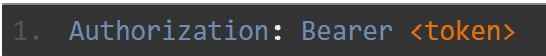
\includegraphics[width = 14cm]{Graphics/bearer_token.jpg}
	\caption{Encabezado de Bearer Toke. }
	\label{fig:bearer_tokne}
\end{figure}

\section{Despliegue:}

\brackcite{carzaniga1998characterization}El despliegue de un sistema es, de manera informal, es el conjunto de procesos a llevar a cabo para poder hace que un software esté disponible para su uso. Aunque esta definición informal define de forma bastante intuitiva el objetivo de despliegue, la estrategia adoptada está vinculada a las especificidades del proyecto que se quiere desplegar. Debido a esto, el desarrollo de una estrategia varía de un sistema a otro.
\newline


\brackcite{pressman2019software}El proceso de despliegue está caracterizado por tres actividades fundamentales: entrega, soporte y retroalimentación. Debido a que en la actualidad los sistemas desarrollados son de carácter incremental y evolutivo, el despliegue ocurre no solo una vez, sino que se lleva a cabo varias veces durante la vida útil del software. Las etapas se pueden caracterizar de la siguiente forma:

\begin{itemize}
	\item \textbf{Entrega:} Cada ciclo de entrega provee al cliente y a los usuarios nuevas características funcionales, incrementando así la operabilidad del software.
    \item \textbf{Soporte:} En los ciclos de soporte se provee documentación y asistencia humana sobre todas las funcionalidades y característica introducidas en todos los ciclos hechos hasta la actualidad.
    \item \textbf{Retroalimentación:} El equipo de desarrollo recibe información y guías para realizar modificaciones de las funcionalidades, características y estrategias a tener en cuenta para la próxima etapa de desarrollo.
    
\end{itemize}

El trabajo requerido para desplegar una aplicación solía ser engorroso y podía requerir gran experticia para lograrlo correctamente. Era un proceso propenso a errores y las actualizaciones eran igual de costosas, lo que hacía más difícil la actualización del sistema y restringía bastante la libertad de los desarrolladores. 
\newline

En la actualidad se ha popularizado el uso de contenedores como substituto de las máquinas virtuales.
\brackcite{docker} Un contenedor es una unidad estándar de software que empaqueta código y todas sus dependencias de forma que la aplicación pueda ser ejecutada rápida y de manera fiable en entornos distintos. Los contenedores y las máquinas virtuales tienen beneficios similares, pero distinto funcionamiento. Los contenedores virtualizan el sistema operativo en vez del hardware, esto los hace más portables y eficientes.
\newline

La herramienta más utilizada para crear y administrar contenedores en la actualidad es Docker, esta facilita el despliegue de aplicaciones ya que solo necesitamos un maquina con Docker para poder correr nuestro contenedores.

\subsection{Docker:}

Es una herramienta para crear y gestionar contenedores. Con la ayuda de Docker los equipos de desarrollo pueden tener confianza en el producto que entregan. Al entregar software contenerizado sabemos que no necesitaremos de configuraciones engorrosas ni manejar errores de despliegue, ya que solo con  tener Docker instalado en la máquina que servirá como host, podemos ejecutar cualquier sistema contenerizado con esta herramienta. Otra de las ventajas evidentes de Docker son los dockerfile, lo cual nos permite escribir de manera secuencial los pasos a seguir para crear un container de un sistema y convertirlo en una imagen ejecutable de Docker. Cada proyecto tiene una forma específica de escribir el dockerfile, en el caso de nuestra implementación, la img \ref{fig:dockerfile} muestra la definición de este archivo:
\newline
\begin{figure}
	\centering
	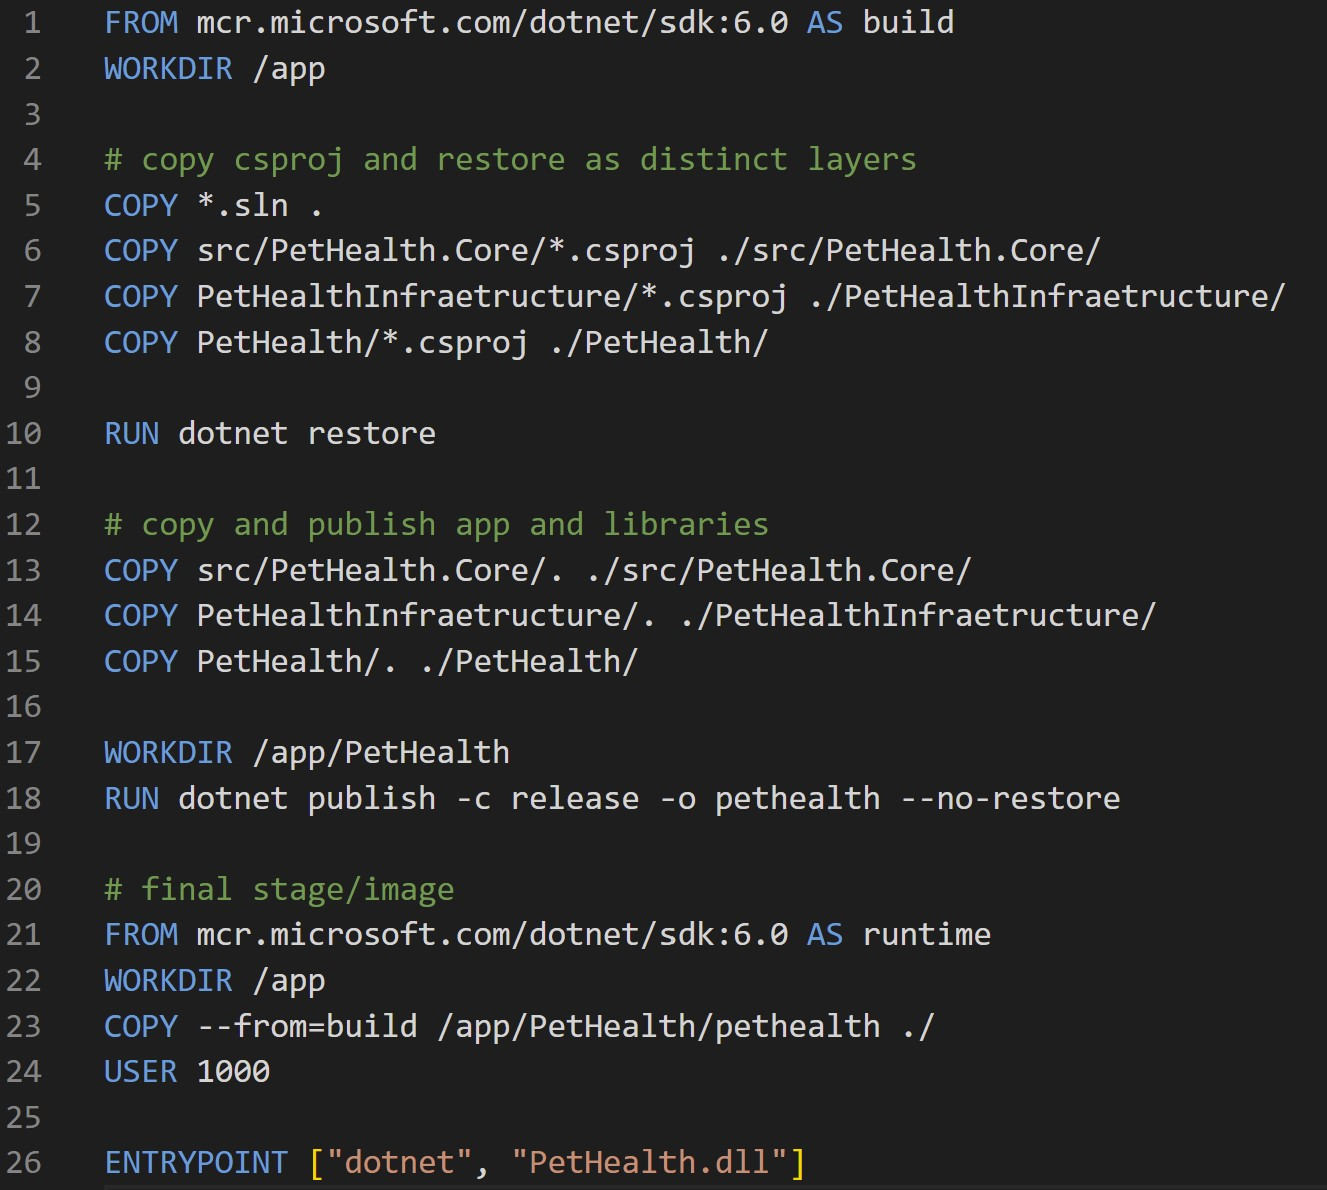
\includegraphics[width = 14cm]{Graphics/dokerfile.jpg}
	\caption{Dokerfile para .NET web api. }
	\label{fig:dockerfile}
\end{figure}

Como podemos ver hemos contenerizado nuestra aplicación en unos cuantos pasos y ya es un contenedor listo para ser ejecutado en cualquier máquina con Docker en ella.

\subsection{Mogenius:}

Mogenius es una herramienta web que automatiza todo el proceso de despliegue y de host de una aplicación. Tiene además la funcionalidad de crear automáticamente un pipeline de CI/CD(Continue Integration/ Continue Deployment), de esta forma nuestra aplicación puede ser fácilmente actualizada sin necesidad de llevar a cabo repetidamente el engorroso desplegar la aplicación. La única configuración necesaria es proveer un archivo dockerfile el cual contenga las instrucciones para contenerizar nuestra aplicación. Este servicio está conectado a una rama especifica del repositorio del proyecto en Gitub, lo que significa que cada vez que sea actualizada la rama principal, la aplicación será desplegada automáticamente sin necesidad de interferir en el proceso. Otra de las ventajas de que el servicio esté conectado a Github, es que podemos controlar las versiones de la aplicación a través de comandos de Git.